
%导言区
\documentclass{article}%book,report,letter

\usepackage{ctex}
\usepackage{fontspec}
%\usepackage{color}
\usepackage{graphicx} %use graph format
\usepackage{subfigure}
\usepackage{epstopdf} %eps图片
\usepackage{amsmath}  %字体加粗
%\usepackage{math}
\usepackage{amsthm}
%制作页眉页脚
\usepackage{fancyhdr}  
\pagestyle{fancy}  
\lhead{第四周作业}  
\chead{微分方程数值解法}  
\rhead{桑明达 15300180062}  
\lfoot{}  
\cfoot{\thepage}  
\rfoot{}  
\renewcommand{\headrulewidth}{0.4pt}  
\renewcommand{\footrulewidth}{0.4pt} 

%标题
\author{names}
\title{\heiti 微分方程数值解法\\ [2ex] \begin{large} 第四周作业 \end{large}}
\author{\kaishu 桑明达 15300180062}
\date{\today}

% 正文区
\begin{document}
\maketitle

%\newpage

\section{P69 1 隐式Euler格式是一阶收敛的}

\begin{proof}
	$ e_{n+1}=u(t_{n+1})-u_{n+1} $,代入隐式Euler格式,有
\begin{align*}
	\left| e_{n+1} \right| = & \left| u(t_{n+1}) - u_n - \Delta t f_{n+1} \right| \\
	 \leq & \left| u(t_{n+1}) - u(t_n) - \Delta t f(t_{n+1},u_{n+1}) \right| + \left| u(t_{n}) - u_n  \right| \\
	& + \left| \Delta t f(t_{n+1},u(t_{n+1})) - \Delta t f(t_{n+1},u_{n+1}) \right| \\
	\leq & \left| R_{n+1} \right| + \left| e_{n}  \right| + \Delta t L \left| e_{n}  \right| \\
	= & \left | \frac{u'' (\xi)}{2}\Delta t^2 \right | + (1+\Delta t L) \left| e_{n}  \right| \\
	\leq  &\frac{M}{2}\Delta t^2  + (1+\Delta t L) \left| e_{n}  \right| \\
	\text{由递推关系,有} \\
	\left| e_{n+1} \right| \leq & \frac{M}{2} \Delta t^2 \frac{(1+\Delta tL)^{n+1}-1}{\Delta t L} + (1+\Delta t L)^{n+1} \left| e_{n}  \right| \\
	\leq & e^{LT}(\frac{M}{2L}\Delta t + \left| e_{0}  \right|  ) 
\end{align*}
\end{proof}

\section{P69 2 四种Euler格式计算$\frac{du}{dt} = au$}

如图\ref{Fig:1},四种Euler格式都是收敛的。
  
\begin{figure}
		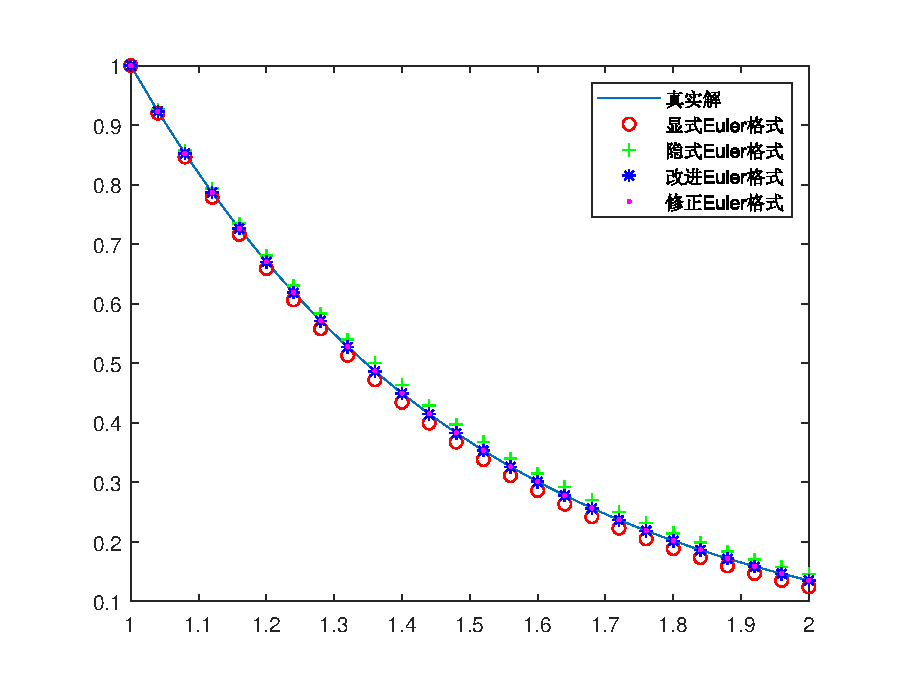
\includegraphics[width=1\linewidth]{week4_2_1.eps}
		\caption{四种Euler格式计算$\frac{du}{dt} = au$}  
		\label{Fig:1}
\end{figure}

\section{P73 1 改进,修正的Euler格式的稳定性分析和绝对稳定区间}

\begin{proof}
	
	对于改进Euler格式,有
	
	\begin{align*}
	\left| u^{\epsilon}_{n+1}-u_{n+1} \right| & =\left| u^{\epsilon}_{n}-u_{n}\right|\left|\frac{1+\frac{a\Delta t}{2}}{1-\frac{a\Delta t}{2}}\right| \\
	&= \left| u^{\epsilon}_{0}-u_{0}\right|{\left| \frac{1+\frac{a\Delta t}{2}}{1-\frac{a\Delta t}{2}}  \right|}^{n} \\
	& ={\left| \frac{1+\frac{a\Delta t}{2}}{1-\frac{a\Delta t}{2}}  \right|}^{n}{\epsilon}
	\end{align*}
	
	希望初始的舍入误差可以控制,则
	
	\begin{align*}
	\left| \frac{1+\frac{a\Delta t}{2}}{1-\frac{a\Delta t}{2}}  \right| & \leq 1 \\
	\left| \frac{1+\frac{z}{2}}{1-\frac{z}{2}}  \right| & \leq 1
	\end{align*}

	对于修正Euler格式,希望初始的舍入误差可以控制,则
	
\begin{align*}
\left | 1+a\Delta t\left (1+\frac{a\Delta t}{2}\right ) \right |& \leq 1  \\
\left | 1+z+\frac{z^2}{2} \right | |& \leq 1 
\end{align*}
\end{proof}

\section{P74 1 Taylor级数计算$\frac{du}{dt}=u-u^2$}

q=2时,有

\begin{align*}
F & =\left ( u-u^2 \right )\left ( 1-2 u \right ) \\
u_{n+1} & =u_{n}+\Delta t \left ( f+\frac{\Delta t}{2} F\right ) 
\end{align*}

q=3时,有

\begin{align*}
G & =\left ( u-u^2 \right )^{2}\left ( -2 \right ) \\
u_{n+1} & =u_{n}+\Delta t \left ( f+\frac{\Delta t}{2} F\right ) +\frac{\Delta t^2 \left ( G+f'_{u}F \right )}{6}
\end{align*}

如图\ref{Fig:2}

\begin{figure}
	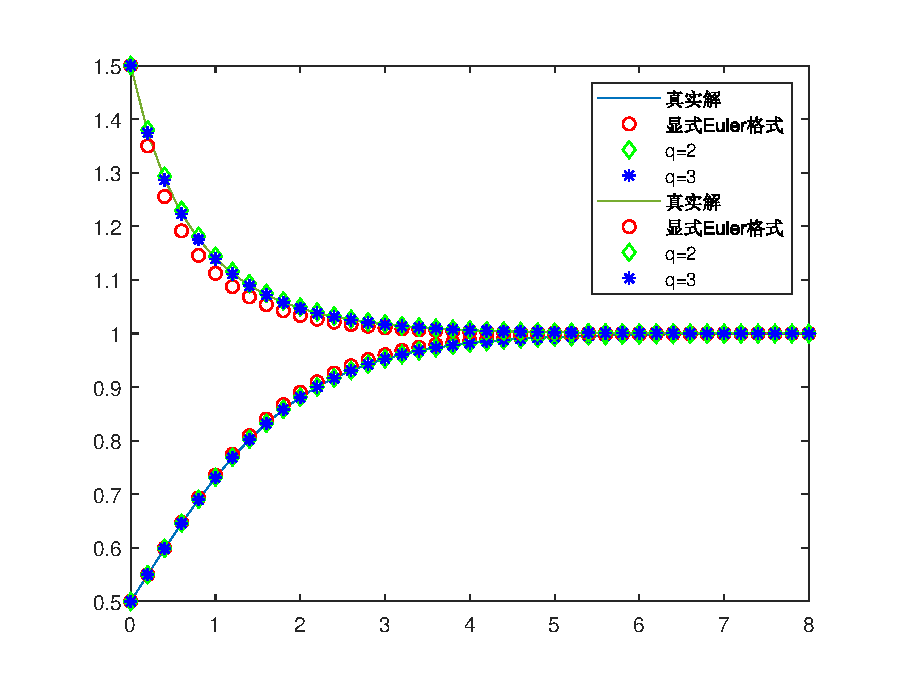
\includegraphics[width=1\linewidth]{week4_4_1.eps}
	\caption{Taylor级数计算$\frac{du}{dt}=u-u^2$}  
	\label{Fig:2}
\end{figure}

\section{P79 2 例2.3.1}

如图\ref{Fig:3}、图\ref{Fig:4}

\begin{figure}
	\includegraphics[width=1\linewidth]{week4_5_1.eps}
	\caption{收敛阶}  
	\label{Fig:3}
\end{figure}

\begin{figure}
	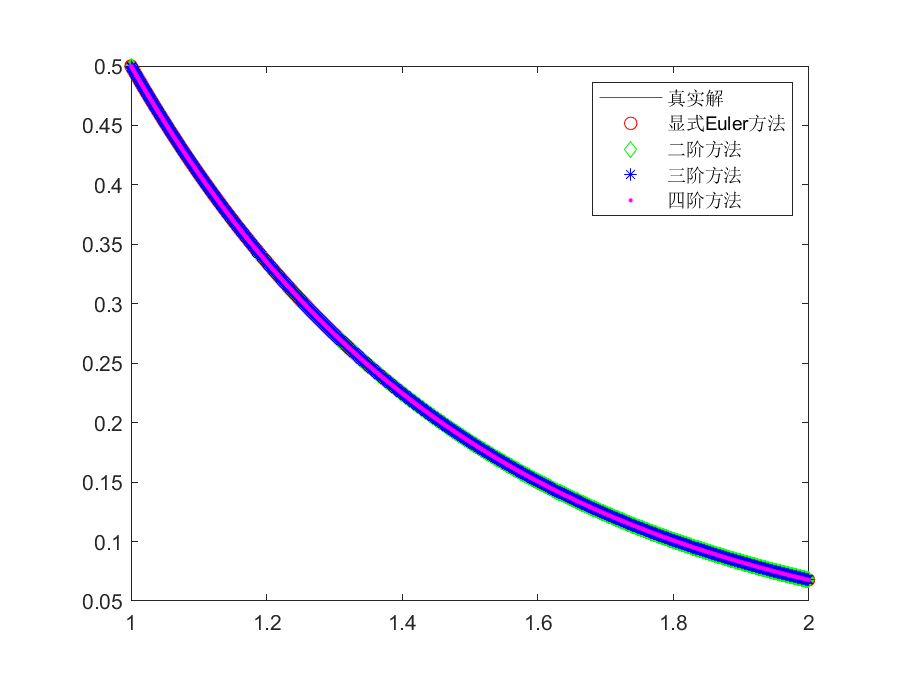
\includegraphics[width=1\linewidth]{week4_5_2.eps}
	\caption{所求函数图像}  
	\label{Fig:4}
\end{figure}

\section{P79 3 例2.2.2}

如图\ref{Fig:5}、图\ref{Fig:6}

\begin{figure}
	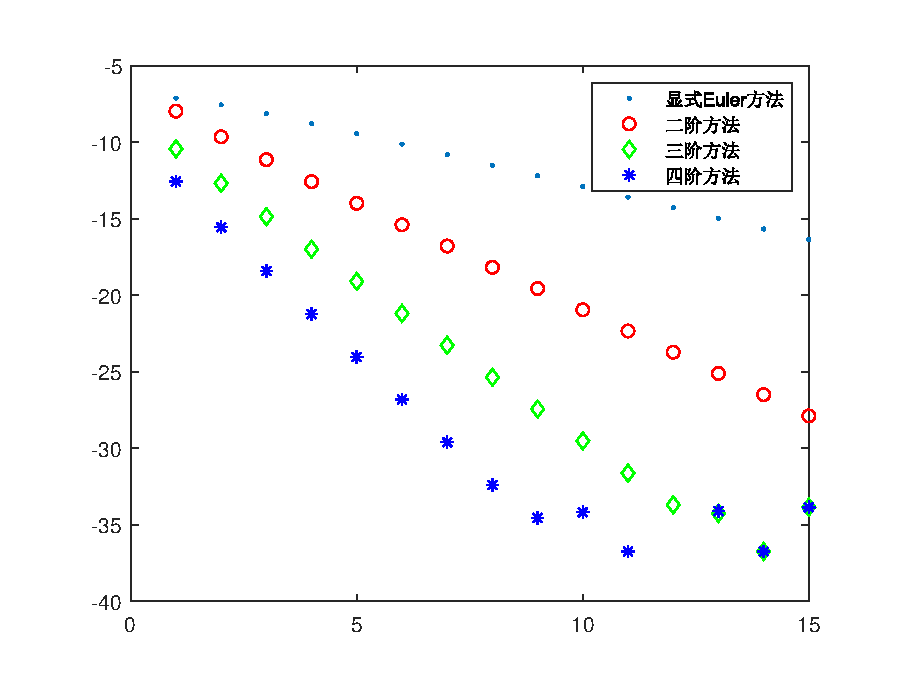
\includegraphics[width=1\linewidth]{week4_6_1.eps}
	\caption{收敛阶}  
	\label{Fig:5}
\end{figure}

\begin{figure}
	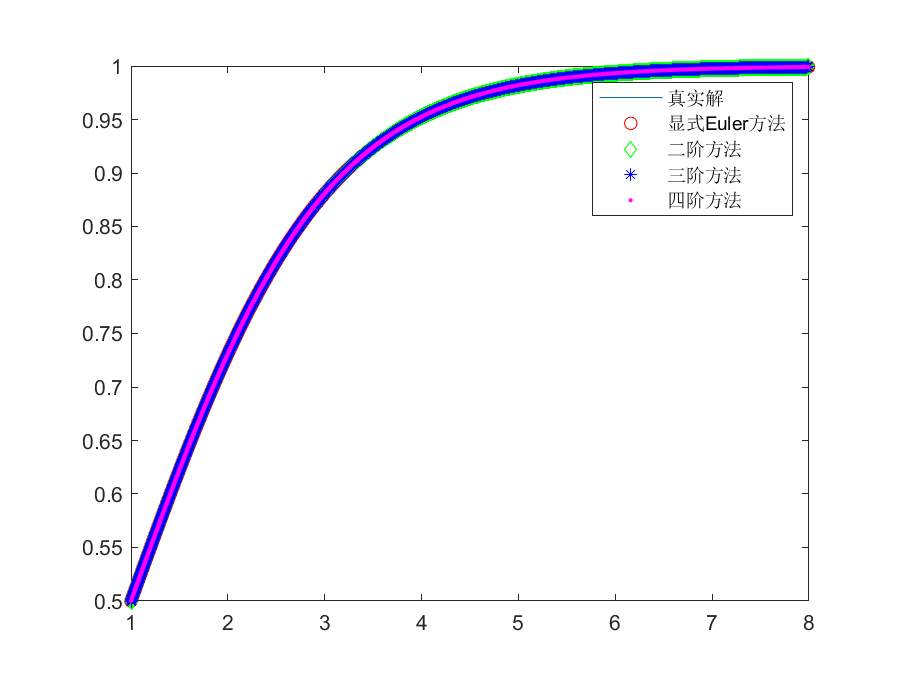
\includegraphics[width=1\linewidth]{week4_6_2.eps}
	\caption{所求函数图像}  
	\label{Fig:6}
\end{figure}

\end{document}